\documentclass[11pt]{article}

\usepackage{graphicx}
\usepackage{wrapfig}
\usepackage{url}
\usepackage{wrapfig}
\usepackage{color}
\usepackage{marvosym}
\usepackage{enumerate}
\usepackage{subfigure}
\usepackage{tikz}
\usepackage{amsmath}
\usepackage{amssymb}
\usepackage{hyperref} 


\oddsidemargin 0mm
\evensidemargin 5mm
\topmargin -20mm
\textheight 240mm
\textwidth 160mm



\newcommand{\vwi}{{\bf w}_i}
\newcommand{\vw}{{\bf w}}
\newcommand{\vx}{{\bf x}}
\newcommand{\vy}{{\bf y}}
\newcommand{\vxi}{{\bf x}_i}
\newcommand{\yi}{y_i}
\newcommand{\vxj}{{\bf x}_j}
\newcommand{\vxn}{{\bf x}_n}
\newcommand{\yj}{y_j}
\newcommand{\ai}{\alpha_i}
\newcommand{\aj}{\alpha_j}
\newcommand{\X}{{\bf X}}
\newcommand{\Y}{{\bf Y}}
\newcommand{\vz}{{\bf z}}
\newcommand{\msigma}{{\bf \Sigma}}
\newcommand{\vmu}{{\bf \mu}}
\newcommand{\vmuk}{{\bf \mu}_k}
\newcommand{\msigmak}{{\bf \Sigma}_k}
\newcommand{\vmuj}{{\bf \mu}_j}
\newcommand{\msigmaj}{{\bf \Sigma}_j}
\newcommand{\pij}{\pi_j}
\newcommand{\pik}{\pi_k}
\newcommand{\D}{\mathcal{D}}
\newcommand{\el}{\mathcal{L}}
\newcommand{\N}{\mathcal{N}}
\newcommand{\vxij}{{\bf x}_{ij}}
\newcommand{\vt}{{\bf t}}
\newcommand{\yh}{\hat{y}}
\newcommand{\code}[1]{{\footnotesize \tt #1}}
\newcommand{\alphai}{\alpha_i}

\pagestyle{myheadings} 



\title{Natural Language Processing: Homework 3}
\author{Name:Yibing Zhang   JHED ID: yzhan316 }
 

\begin{document}
\large
	\maketitle
	\thispagestyle{headings}
	
	\vspace{-.5in}


	
	\paragraph{1}.\\
\\
(a)\\
\\
I participated a party held by Jimmy.\\
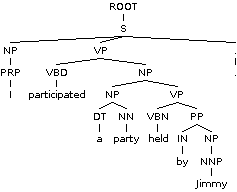
\includegraphics[width=0.8\linewidth]{parse1.png}\\
\\
I received the best gift that I have ever received.\\
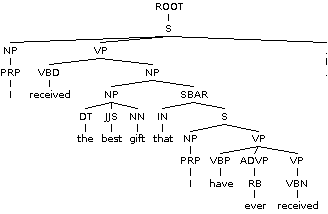
\includegraphics[width=0.8\linewidth]{parse2.png}\\
\\
could you please tell me the time when we are supposed to hand in this assignment?\\
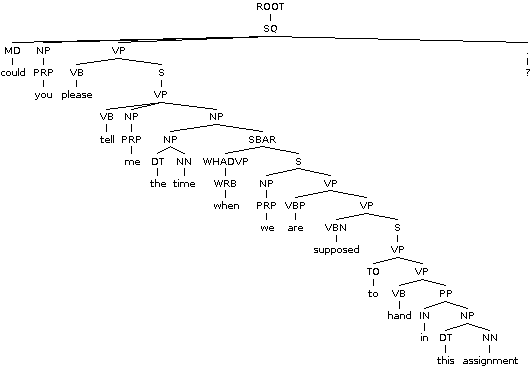
\includegraphics[width=0.8\linewidth]{parse3.png}\\
\\
That is what annoys me a lot.\\
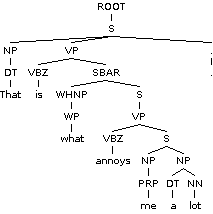
\includegraphics[width=0.8\linewidth]{parse4.png}\\
\\
As we can see, there are more non-terminals than we previously learned, depending on the tenses, single or plural and so on. 
And there are lots of preterminals defined before the terminals come out.\\
\\
(b)\\
There are also some places not satisfying. For example, in the fourth parsing, ''me a lot'' was parsed as a ''S'' which was composed of two NPs.\\
\\
And there is a grammar NP $\rightarrow$ DT, which means a determiner itself could be a NP, just like ''that'' in the fourth parsing above.\\
\\
Also, ''hand in this assignment'' is parsed as \\
VP (VB hand)
      (PP (IN in)
            (NP (DT this) (NN assignment))).\\
However, we know that ''hand in'' should be interpreted as a verb phrase.\\
\\
The parser tried to recognize relative clauses in a relatively complex sentence.\\
In addition, it differentiates adjectives as normal, comparative and superlative. It also detects tenses of verbs.\\
\\
(c)\\
example:  What should I hand in in this assignment?\\
result:\\
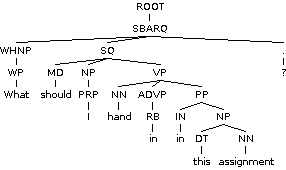
\includegraphics[width=0.8\linewidth]{parse5.png}\\
\\
As we can see, the parse still cannot parse the verb phrase ''hand in''. What's worse, ''hand'' is interpreted as a ''NN''(Noun).\\
\paragraph{3}. \\
\\
(a)\\
Results for gen/*\\
176 files were more probably gen (97.78\%)\\
4 files were more probably spam (2.22\%)\\
\\
Results for spam/*\\
61 files were more probably gen (67.78\%)\\
29 files were more probably spam (32.22\%)\\
\\
Thus, the error rate is $\frac{4+61}{180+90}=24.07\%$\\
\\
(b)\\
When I set the prior probability as $10^{-323}$, which is the smallest value a log function can take, there are still 1 file in gen/* and 2 files in spam/* classified as gen.\\
\\

(c)\\
As for gen, when $\lambda=0.00852$, the cross-entropy per token is the minimum. The minimum is 8.74253\\
As for spam, when $\lambda=0.014$, the cross-entropy per token is the minimum. The minimum is 7.10009.

(d)\\
Cross-entropy per token$=\frac{Total~cross-entropy~on~/dev/gen/*+Total~cross-entropy~on~/dev/spam/*}{count(tokens~in~/dev/gen/*)+count(tokens~in~/dev/spam/*)}$\\
When $\lambda^*=0.01$, the cross-entropy per token on the whole dev set reach its minimum, which is 8.0104\\
\\

(e)\\
To solve this problem, I wrote a program named ''sortOnLength.py''. This program will will sort our classification result on dev set on lengths of files.
For example, there are a few lines in our classification result of dev/spam/*:\\
gen	./gen\_spam/dev/spam/spam.78.025.txt\\
spam	./gen\_spam/dev/spam/spam.80.011.txt\\
spam	./gen\_spam/dev/spam/spam.8.081.txt\\
spam	./gen\_spam/dev/spam/spam.81.087.txt\\
\\
Then my program will sort and print the result as:\\
(8,78)   (80,81)\\
 0.5    \hspace{1cm}          1.0\\
(8,78) means files of length from 8 to 78. And 0.5 means the classification accuracy on files of length from 8 to 78.\\
To run my program, I firstly output the classification results of dev/gen/* and dev/spam/* in result\_gen and result\_spam respectively. Then put those two results in the same directory as my program. Then, just run by typing ''python3 ./sortOnLength.py''.\\
In addition, the number of files in per length range to calculate the accuracy is 13.
The table below describes the relationship between lengths and accuracies($\lambda=0.01$, prior probability of gen is 0.7).\\
\begin{tabular}{|c|c|} 
\hline 
Length&Accuracy\\
\hline  
(5, 20)&0.6\\
\hline
(22, 35)&0.875\\
\hline
(37, 55)&1.0\\
\hline
(57, 69)&0.929\\
\hline
(71, 89)&0.857\\
\hline
(91, 98)&0.857\\
\hline
(104, 118)&0.933\\
\hline
(121, 134)&0.929\\
\hline
(141, 161)&0.933\\
\hline
(164, 180)&0.929\\
\hline
(183, 211)&0.857\\
\hline
(218, 253)&0.786\\
\hline
(266, 290)&1.000\\
\hline
(299, 331)&0.929\\
\hline
(345, 449)&0.929\\
\hline
(457, 660)&0.786\\
\hline
(700, 1209)&0.786\\
\hline
(1355, 8185)&0.500\\
\hline
\end{tabular}\\
And the graph below is drawn based on the table.\\


(f)\\

\paragraph{4}.\\
(a)\\
If $V=19999$, then in uniform estimate, $\sum_z \hat{p}(z\mid x y)=\frac{20000}{19999}>1$,which is incorrect. Similarly, in ADDL estimate, $\sum_z \hat{p}(z\mid x y)=\frac{\sum_z (c(xyz)+\lambda)}{c(xy)+\lambda V}=\frac{c(xy)+20000\lambda}{c(xy)+19999\lambda}>1$,which is incorrect too.\\
(b)\\
If $\lambda=0$, then $\hat{p}(z\mid x y)=\frac{c(xyz)}{c(xy)}$, which has no smoothing at all. Without smoothing, the probability of many files with unseen words will become zero.\\
(c)\\
In BACKOFF\_ADDL, if $c(xyz)=c(xyz')=0$, $\hat{p}(z\mid x y)=\frac{c(xyz)+\lambda V \hat{p}(z\mid y)}{c(xy)+\lambda V}=\frac{\lambda V \hat{p}(z\mid y)}{c(xy)+\lambda V}$.\\
Similarly, $\hat{p}(z'\mid x y)=\frac{\lambda V \hat{p}(z'\mid y)}{c(xy)+\lambda V}$.\\
if $\hat{p}(z\mid y)\neq \hat{p}(z'\mid y)$ , then $\hat{p}(z\mid x y)\neq \hat{p}(z'\mid x y)$\\
When $c(xyz)=c(xyz')=1$, $\hat{p}(z\mid x y)=\frac{1+\lambda V \hat{p}(z\mid y)}{c(xy)+\lambda V}$, $\hat{p}(z'\mid x y)=\frac{1+\lambda V \hat{p}(z'\mid y)}{c(xy)+\lambda V}$.\\
So, if $\hat{p}(z\mid y)\neq \hat{p}(z'\mid y)$ , then $\hat{p}(z\mid x y)\neq \hat{p}(z'\mid x y)$\\

(d)\\
$\lambda$ defines how much it smoothes the probabilities using $\hat{p}(z\mid y)$. Larger $\lambda$ will make $\hat{p}(z\mid x y)$ closer to $\hat{p}(z\mid y)$\\
\\


\paragraph{5}.\\
The $\lambda^*$ I used here is 0.01\\
\\

\paragraph{6}.\\
(c)\\
\begin{tabular}{|c|c|c|} 
\hline 
C&Cross-entropy&Accuracy\\
\hline  
1&4.384&0.799\\
\hline
0.05&4.405&0.791\\
\hline
0.1&4.404&0.791\\
\hline
2&4.368&0.795\\
\hline
3&4.357&0.799\\
\hline
4&4.349&0.803\\
\hline
5&4.343&0.803\\
\hline
6&4.339&0.803\\
\hline
7&4.337&0.795\\
\hline
8&4.335&0.795\\
\hline
10&4.334&0.795\\
\hline
\end{tabular}\\
As we can see, when $C=5$, the classification accuracy become the highest.\\ 
Thus, $C^*=5$.\\
\begin{tabular}{|c|c|c|} 
\hline 
embeding&Cross-entropy&Accuracy\\
\hline  
10&4.343&0.803\\
\hline
20&4.199&0.849\\
\hline
40&4.125&0.849\\
\hline
\end{tabular}\\
\\
The more dimensions we have in our word embedding, the more information we can know about a word, which means we have more features to use. Thus, the accuracy increases and the cross entropy decreases.\\
I use training data to build my model, to tune parameters in matrices $X,Y$ using SGD. And I use dev data to tune the hyperparameter $C$ and also dimension of word embedding. And test data can be used to compare the accuracy of my loglinear model with that of the add-$\lambda$ back-off model.\\
\\
When I was tuning $C$, I found that when I got the $C$ which could produce the highest accuracy, it was not the $C$ that could produce the minimum cross-entropy.That is because in order to predict the correct label, your probability does not need to be very big. It just need to be bigger than the probability of the other label. So, the cross entropy may not be the minimum when the accuracy is the highest.\\
\\
To compare the result with that of add\_$\lambda$ back-off,\\
I set $\lambda^*=0.01, C=5$, dimension=20. Below is the comparison.\\
Backoff\_add:\\
Accuracy: 0.854\\
Cross-entropy per token: 5.148\\
\\
Loglinear model:
Accuracy: 0.849\\
Cross-entropy per token: 4.199\\
\\
As we can see, the accuracy of backoff\_add$\lambda$ is a little bit higher. However the cross entropy of backoff\_add$\lambda$ is lower, which means even though it can predict the correct label, it is not so confident on that.\\
\\
(d)
I implemented the unigram log-probability.\\
\\
\paragraph{7}.\\
Just find the $\vec{w'}$ that maximizes $P(\vec{w'}\mid U)$. And according to Bayes theorem, $P(\vec{w}\mid U)=\frac{P(\vec{w})P(U\mid \vec{w})}{P(U)}$. Since we already know $P(U\mid \vec{w})$ and we can estimate $P(\vec{w})$ using our language model. We don't need to know the denominator because we only need to find the $\vec{w'}$ that maximizes $P(\vec{w'})P(U\mid \vec{w'})$, which is equivalent to maximizing $P(\vec{w'}\mid U)$.\\


\end{document}
